\section{问题提出的背景}

\subsection{背景介绍}

\subsubsection{现实背景}

随着现代多核处理器的发展,目前无论是移动设备,还是桌面设备、服务器,都广泛的配备了多核处理器,这使得并发编程越来越重要。但这也带来了新的问题,就是并发漏洞的检测和修复。并且由于现代程序越来越复杂,仅仅针对普通程序的检测手段已经无法有效检测到高度复杂的并发漏洞。同时由于并发漏洞本身是由于非确定的线程调度导致的,即使成功触发了并发漏洞,但是在之后还是很难对漏洞进行定位和修复。这对高效的并发漏洞检测工具提出了要求,传统的测试技术逐渐被淘汰,现在模糊测试作为时兴的技术,将模糊测试技术应用到并发漏洞发掘领域有助于快速检测程序中的漏洞,避免造成损失。

\subsubsection{技术与问题背景}

\paragraph{竞争条件}竞争条件是指电子设备、软件或者其他系统的实质性行为取决于其他不可控时间的顺序或者时间,从而导致意外或者不一致的结果。如果其中一种或者多种行为是不能接受的情况,它就会成为一个漏洞\cite{wikipediaRaceCondition}。

数据竞争指的是在多线程程序中,两个或两个以上线程对同一个共享的内存地址进行访问,并且其中至少有一个是写操作。如果这样的操作没有正确地用锁或者其他机制进行保护,就会导致数据竞争的出现。例如当两个线程同时想要修改一个变量时,可能会出现以下的两种情况,第一种情况下可以对值进行正确的修改,第二种情况下由于不正确的运行顺序,会导致值最终的结果和预期不符合。

\autoref{fig:fig2}为第一种情况,首先线程1从内存中读取值,然后执行加1操作,然后再写回到内存中。然后线程2执行同样的步骤,最终值为2。

\begin{figure}[ht]
    \centering
    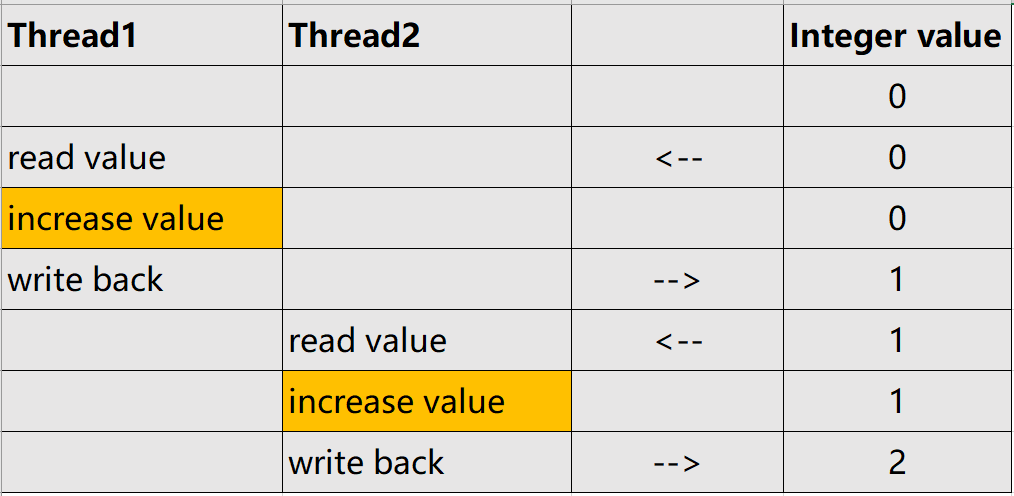
\includegraphics[width=0.8\linewidth]{fig2}
    \caption{\label{fig:fig2}正确的并发访问}
\end{figure}

\autoref{fig:fig3}为第二种情况,这种情况下,首先线程1和线程2分别从内存中读取对应的值0,然后各自进行加1操作,此时两者的值都为1,最后两个线程分别将自己加1得到的值写回内存中,因此最终内存中的值为1。这里产生了数据争用,由于线程交错,导致两者错误地得到值并修改,最终将不符合预期的值写回到内存中,导致了错误。

\begin{figure}[ht]
    \centering
    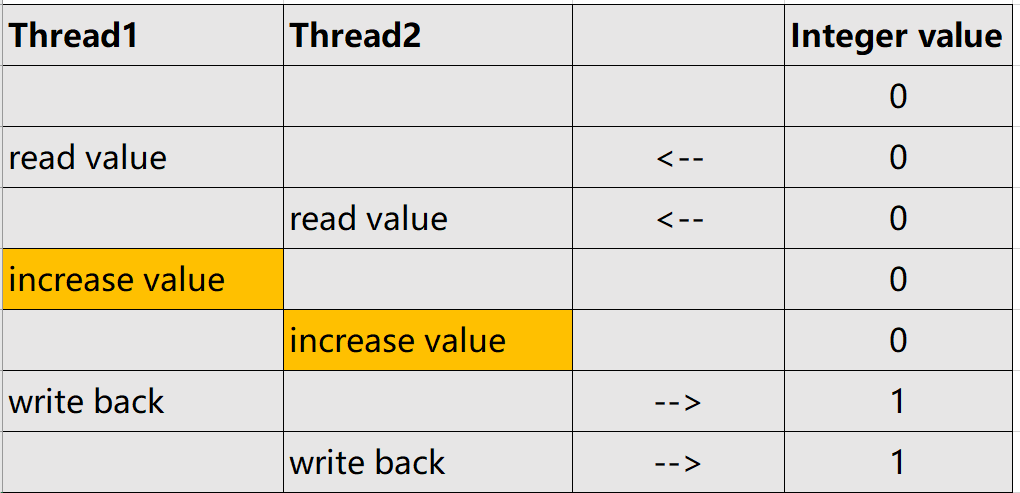
\includegraphics[width=0.8\linewidth]{fig3}
    \caption{\label{fig:fig3}错误的并发访问}
\end{figure}

避免数据竞争主要要求程序员在编写多线程程序时严格遵守一些规则和原则包括但不限于同步,有序性和原子性。避免数据竞争的策略目前有很多,例如:

\begin{enumerate}
\item 首先,可以使用锁定机制确保任何时候只有一个线程访问数据。在执行读写操作之前,线程必须获得锁,读写完成后解锁。这样其他所有尝试获取锁的线程就会被阻塞,直到持有锁的线程完成操作。这种方法可以有效的防止数据竞争,但也可能导致锁竞态和性能问题。
\item 其次,可以使用原子操作确保操作不受线程切换影响。所谓的原子操作,就是在执行中不会被线程切换打断的操作。一些编程语言提供了对原子操作的支持,如C++11中的std::atomic。
\item 然后,另一种策略是设计无共享数据的程序。既然数据竞争是由于多个线程同时访问同一块数据,那么避免共享数据就可以避免数据竞争。这种策略有时候被称为消息传递,其中线程之间通过发送消息来交换信息。每个线程有自己的数据副本,因此不存在数据竞争。然而,这种方法可能会增加数据复制和通信的成本。
\item 最后,可以使用一些诸如事务性内存的较新的并发控制技术。在事务内存模型中,一组读取和写入被组合在一个事务中,只有当没有其他线程访问被事务使用的数据时,这个事务才能成功提交。
以上就是防止数据竞争的一些常见策略和技术。谨记,无论使用哪种策略,在编写并发代码时,始终需要注意数据访问的顺序和时机,以及线程如何互相影响。
\end{enumerate}

\paragraph{模糊测试}模糊测试(Fuzz testing 或 Fuzzing)是一种软件测试技术,它通过自动或半自动方式向系统提供无效、意外或随机的数据,并监控系统的响应,从而查找可能的错误和漏洞。模糊测试是通过大量的输入测试来检查程序是否存在异常状况,比如崩溃或者未捕获的异常,是一种健壮性测试。模糊测试包括几个主要的步骤:

\begin{enumerate}
\item 确定目标:首先确定测试的目标,也就是要测试的软件或者系统。可以是一个网络协议,一个文件格式,或者一个具体的功能。
\item 生成模糊数据:这个步骤是通过不同的方法生成一些随机或伪随机的数据作为输入。可以是完全随机的数据,也可以基于一些规则或者模型生成。有些高级的模糊测试工具还能够理解输入的结构,并基于这个结构生成更有效的模糊数据。
\item 执行并监控:将这些模糊数据输入到被测试系统,监控系统的行为。如果系统出现异常,如崩溃或者挂起,那么就可能存在问题。
\item 分析结果:对每一个引发异常的输入数据进行分析,确定这是一个真实的漏洞,还是一个假阳性。如果是一个真实的漏洞,那么就需要进一步调查并修复。
\end{enumerate}

模糊测试是一种强大的测试方法,尤其在安全测试领域。它能够找到一些传统的测试方法很难发现的问题。通过模糊测试,可以发现和修复应用程序中的可利用漏洞,进而增强系统的稳定性和安全性。

\subsection{本研究的意义和目的}

根据\cite{cvedetailsSecurityVulnerability}可以看出,当前的漏洞种类中有关并发程序的越来越多,这是因为多核处理器的不断发展以及并发编程模式的广泛应用,尽管在并发编程中有很多指导性的原则,但是在程序员进行实际的开发时还是难免会写出带有并发访问漏洞的程序。即使是在一些拥有高度活跃的开发者社区的项目同样有可能产生这些错误,因此能够在开发阶段将这些错误成功检测出来并给出详细的报告是很有必要的,这有助于开发者将在早期将潜在的威胁消除,防止使用者受到攻击。由于模糊测试的本质是生成随机输入测试系统是否能够正常运行,利用模糊测试不仅仅可以检测出常规手段不能检测出来的漏洞,还可以进一步检测系统的鲁棒性和稳定性。但在利用模糊测试挖掘漏洞上目前的研究取得了比较好的效果,因此通过对模糊测试系统进行调整和加强,使其能够在并发漏洞的挖掘上更加有效是很有意义和前景的工作,是有价值的。